%Linea Para poder completar automaticamente las citas con el Sublime
%No hace el documento, se puede borrar esta linea si no se usa el Sublime
%------------------------------------------------------------------------------
 \newcommand{\NoBiblioEQ}[1]{
 \ifthenelse{\equal{#1}{verdadero}}{}{\bibliography{Referencias/base_bibliografica}}
 \NoBiblioEQ{verdadero}}
 %----------------------------------------------------------------------------- 

%Formato (Nombre de capitulo largo o corto), nombre del capitulo y estilo de la
%Portada del Capitulo
%------------------------------------------------------------------------------

 %Formato en si, titulo en un solo renglon
 \FormatoCapituloDosLineas
 
 %Nombre y etiquete para referir
 \chapter{Electroquímica en películas delgadas mesoporosas}
 \label{chap:Electroquimica}

 %Para que no salga el numero de pagina en la portada del capitulo
 \thispagestyle{empty}
	
 %Resumen del Capitulo en Italica
 \noindent\textit{En este capitulo se estudia exhaustivamente los fenómenos de transporte\index{transporte} de sonda\index{sonda}s a través de las películas delgadas mesoporosas y su respuesta electroquímica\index{electroquimico}. Analizando los resultados obtenidos por voltametría cíclica, voltatametría cíclica\index{voltametria!cíclica} de corriente alterna y simulaciones por elementos finitos, se sugiere un modelo de transporte\index{transporte} para cada caso y se calculan parámetros para los distintos sistemas, como concentración dentro las poros, coeficiente de difusión\index{difusión}, constante de Langmuir\index{Langmuir} y estabilidad química entre otros.}

 %Indice de capitulo alineada al borde inferior de la pagina, nueva pagina
 \vfill
 \minitoc
 \newpage
 %-------------------------------------------------------------------------------

\section{Introducción}

	Una vez estudiados los distintos tratamientos de síntesis y realizada la fabricación de los sensores\index{sensor} se dedicará, en este capitulo, a estudiar las propiedades de los mismos para detectar y cuantificar una serie de sonda\index{sonda}s electroquímica\index{electroquimico}s\index{electroquimico} elegidas, precisamente, para poder evaluar distintos aspectos de transporte\index{transporte} a través de los sistemas nanoporosos. 
	Los sensores\index{sensor} están compuestos básicamente de una película delgada \index{película!delgada}de oro\index{oro} y una película delgada \index{película!delgada}nanoporosa.

	La superficie\index{superficie} de las paredes dejan expuestos, hacia el interior de los poros, grupos silanoles los cuales pueden estar o no protonados.\cite{Brinker1990,Soler-Illia2011} 
			\begin{equation}
				\begin{aligned}
				\includegraphics[scale=0.75]{Esquemas/equilibriosilica.pdf}
				\label{eq:equilibriosilica}
				\end{aligned}
				\end{equation}

	La reacción \ref{eq:equilibriosilica} ejemplifica el equilibrio ácido-base que se establece en la superficie\index{superficie} de la sílice. El pKa del $\text{SiO}_2$ es menor a 4 y la mayoría de los autores coinciden en que el punto isoeléctrico\index{punto isoeléctrico} (PI) varía de $1$ a $4$ dependiendo de  las distintas forma alotrópicas del óxido de silicio\index{silicio!oxido de}, en particular para el SiO$_2$ sintetizado vía sol-gel\index{sol-gel} el $\text{PI}\approx 2$ \cite{Kosmulski2002,Kosmulski2014,Schwarz1984,Si-HanWu2013}.
	Wu\index{Wu} y colaboradores\cite{Si-HanWu2013} analizaron, por un lado, el estado de carga superficial de nanoparticula\index{nanoparticula}s\index{nanoparticula} de sílice mesoporosa\index{película!mesoporosa} y, por otro, la tasa de condensación\index{condensación}. El gráfico de la figura \ref{fig:silica_ph} muestra como varían las razones  $\text{SiO}^{-}/\text{SiOH}$ y $\text{SiOH}_2^{+}/\text{SiOH}$ en función del pH\index{pH}; se puede apreciar que solo por encima de $\text{pH}\geq7$ se obtiene una superficie\index{superficie} de carga negativa donde todos los silanoles reaccionaron, cediendo su $\text{H}^{+}$, para convertirse en iones silanoatos; mientras que para pH\index{pH} bajos ($\text{pH}\leq1$), la sílice se vuelve inestable antes de llegar a un estado de carga completamente positivo y, solo queda, parcialmente positiva. En el mismo trabajo\cite{Si-HanWu2013} también plantean que la tasa de condensación\index{condensación} decrece por encima de $\text{pH}\geq7.5$ debido a que entra en una zona de inestabilidad donde el óxido se disuelve, catalizado por el medio básico.
		\begin{figure}[th!]
			\centering
 	       	\includegraphics[width=0.70\textwidth]{Graficos/Silica-PH-Stability.pdf}
	    	\caption[Tasa de condensación\index{condensación} y estado de carga superficial]{Tasa de condensación\index{condensación} y estado de carga superficial para nanoparticula\index{nanoparticula}s\index{nanoparticula} de sílice en función de pH\index{pH}. Gráfico extraído de \textit{Synthesis of mesoporous silica nanoparticles} Chem. Soc. Rev., 42(9):3862, 2013.\cite{Si-HanWu2013}}
	       	\label{fig:silica_ph}
	    	\end{figure}
	De hecho, Iler\index{Iler}, en su libro \textit{<<The Chemistry of Silica>>}, explica que la tasa de disolución de la sílice en medio acuoso depende de muchos factores y, que además, salvando el tipo de sílice, el proceso de disolución requiere de un catalizador. Presenta un gráfico de la tasa de disolución en función del pH\index{pH} (figura \ref{fig:disolucion_ph}) y postula que la misma depende de la forma alotrópica de la sílice. Para formas mas porosas, como el SiO$_2$ amorfo, la cinética de disolución es mas rápida, mientras que para otras, mas cristalinas, como el cuarzo, se hace mucho mas lenta. Por último aclara que se trata de un proceso de despolimerización vía hidrólisis\index{hidrolisis@hidrólisis}, y que la solubilidad es la concentración de Si(OH)$_4$ cuando alcanza un estado estacionario en el equilibrio despolimerazación-polimerización.\cite{iler1979}. 

			\begin{figure}[th!]
			\centering
 	       	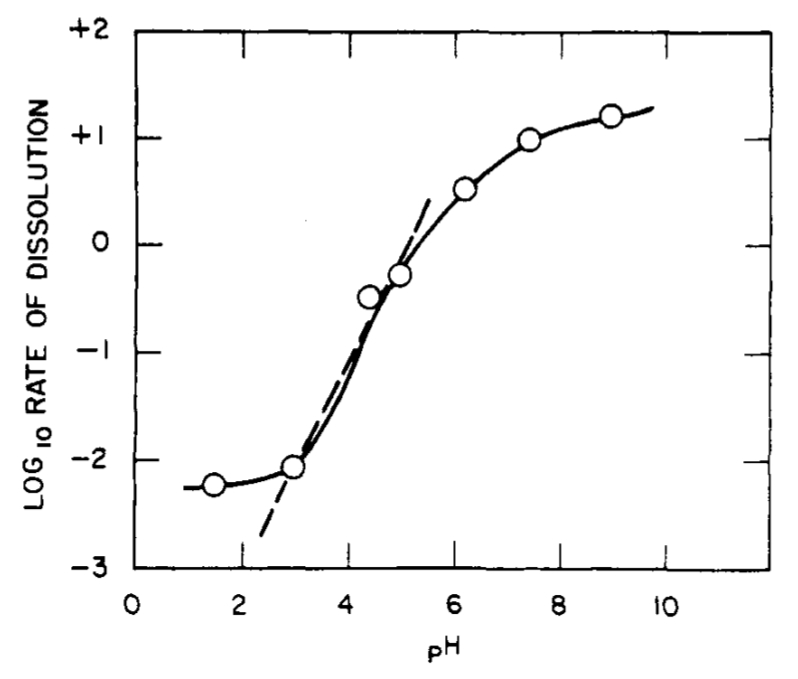
\includegraphics[width=0.70\textwidth]{Graficos/disolucion_ph.pdf}
	       		\caption[Tasa de disolución sílice en función del pH\index{pH}]{Tasa de disolución de la sílice en función de pH\index{pH}. Gráfico extraído de \textit{The chemistry of silica} Wiley 1ª edición, 1979.\cite{iler1979}}
	         	\label{fig:disolucion_ph}
	     		\end{figure}
	
	También propone un mecanismo en medio ácido\index{acido@ácido} catalizado por iones F$^-$, mientras que en medio básico\index{básico} el mecanismo es catalizado por iones OH$^-$, según el siguiente mecanismo:
			\begin{equation}
				\begin{aligned}
				\includegraphics[scale=0.60]{Esquemas/disolucionsilica.pdf}
				\label{eq:disolucionsilica}
				\end{aligned}
				\end{equation} 
	
	El mecanismo de \ref{eq:disolucionsilica} no está completamente consensuado en la literatura especializada, sin embargo todos los autores coinciden en que el óxido se vuelve inestable en cualquiera de sus forma alotrópicas a partir de un $\text{pH}\geq7$ y que, a partir de $\text{pH}\geq10$ el proceso de disolución se acelera varios ordenes de magnitud.\cite{Kosmulski2002,Kosmulski2014,Schwarz1984,Si-HanWu2013,iler1979}

	%Dependencia de la constante de K con el PH.... poner aqui el grafico, ecuacion y grafico de Wu2013 donde propone estado de carga y donde se muestra que recien a PH=5 se llega a un estado de carga copmpeltamente negativo.
	
				
	%ca tengo que poner como es la reaccion del punto isoeléctrico\index{punto isoeléctrico} del Sio2 o del punto de carga zero... o del pka??? Y tambien tengo que poner los antecendente de calvo, calvo y el otro del 2005. Y tambien entonces que la diferencia es el Au\index{oro} miniaturizacion, etc, etc mayores velocidades... etc. 
	%No olvidarse de los ferrocenos a distintas velociades de barrido

\section{Transporte de sonda\index{sonda}s en \pdm}

	 Durante las próximas secciones se analizan e interpretan los resultados obtenidos al colocar soluciones con sonda\index{sonda}s electroquímica\index{electroquimico}s\index{electroquimico}, de diferente naturaleza, sobre los sensores. Al\index{aluminio} ser, la fabricación de los sensores, una parte estructural de este trabajo, cabe aclarar sobre que sistemas se realizaron los experimentos mostrados en este capitulo. Se utilizó, indistintamente, películas de Au\index{oro} sobre sustratos varios (silicio, vidrio, flexible), con diseño ya transferido o sin transferir. En este capitulo se trabajó exclusivamente en sistemas con películas delgadas mesoporosas (\pdm), de óxido de silicio\index{silicio!oxido de}\index{silicio} (\pdmF) o de óxidos mixtos silicio/circonio (\pdmZ), estructuradaras con Pluronic F127\index{Pluronic F127}, y sintetizada con el método de alto vacio\index{alto@alto vacío} (consultar sección \ref{sec:trat-vacio}, pág. \pageref{sec:trat-vacio}). Todas las medidas electroquímica\index{electroquimico}s\index{electroquimico} (EQ) usaron como referencia un electrodo saturado de calomel (ESC) y fueron normalizadas por el área geométrica del electrodo, de forma de facilitar la comparación de resultados cuando se trata de sensores\index{sensor} con distinto diseño. Todas los experimentos fueron llevadas a cabo a $\text{pH}\approx5,5$ en solución de KCl \SI{100}{\milli\Molar}. Esta elección se basa en el doble propósito de elegir un pH\index{pH} que podemos encontrar en sumideros de aguas naturales, y conservar dentro de las películas delgadas mesoporosas una fuerte carga negativa sin comprometer disolución de la sílice.

	\subsection{Caso 1: sonda\index{sonda} de carga negativa}

	 El voltagrama de la figura \ref{fig:exclusion_vs_Au} muestra la respuesta de los sensores\index{sensor} cuando se colocan en una solución con una sonda\index{sonda} negativa. Para este fin se utilizó una solución de ferrocianuro de potasio\index{ferrocianuro de potasio} (\ferroCompleto) y ferricianuro de potasio\index{ferricianuro de potasio} (\ferriCompleto) en proporciones equimolares, que de ahora en mas llamaremos \fe. El voltagrama rojo corresponde a la respuesta en un electrodo de Au\index{electrodo!de Au}\index{oro} desnudo, mientras que la verde a un electrodo recubierto de con una \pdm.
	
			\begin{figure}[ht]
				\centering
		 	    \includegraphics[width=0.70\textwidth]{Graficos/ExclusionFcCN.pdf}
		        \caption[Exclusión electrostática en \pdmF]{Respuesta compartiva de un electrodo de Au\index{electrodo!de Au}\index{oro} recubierto con \pdmF\space y sin recubrir frente a una sonda\index{sonda} \fe\space \SI{1}{\milli\Molar} en \SI{0.1}{\Molar} de KCl contra ESC.}
		        \label{fig:exclusion_vs_Au}
		      	\end{figure}
	
	 Al\index{aluminio} ser la sonda\index{sonda} de carga negativa, no es capaz de ingresar a la película (la cual está cargada negativamente), y, por lo tanto tampoco puede difundir hacia el electrodo, eso se refleja en el voltagrama donde no se observa ni reducción ni oxidación de la sonda\index{sonda}. La repulsión se debe a un efecto de exclusión electrostática. Este fenómeno de exclusión ya fue reportado por varios autores\cite{alberti2015,schmuhl2005,Andrieu-Brunsen2015,brunsen2011}. Al\index{aluminio} pH\index{pH} de trabajo, $\text{pH}=5,5$, los silinanoles están como \index{silanolato}s, como ya se explicó anteriormente, estableciendo una carga negativa en todo el espesor\index{espesor} de la película.

	 Desde el punto del estudio de fenómenos de  transporte\index{transporte} esta sonda\index{sonda} no es especialmente útil, porque, como ya se demostró, no puede ingresar en la \pdm. Sin embargo, nos ofrece información importante sobre la integridad estructural de las películas delgadas, dicho de otro modo, al no obtener señal electroquímica\index{electroquimico} significa que la sonda\index{sonda} no percola a través de la \pdm, que la \pdm\space se encuentra sin fisuras, agujeros o rajaduras y que recubre por completo el área del electrodo.

	 Por ende fue muy importante para corroborar (si no hay señal la \pdm está intacta, si hay señal el Au\index{oro} quedó expuesto) el estado de las \pdm\space al finalizar experimentos donde se dudaba del estado de la película.  De esta forma esta sonda\index{sonda} se utilizó a modo de <<experimento control>> para comprobar que las películas no tuviera sitios de percolación debido a daños estructurales.

	\subsection{Caso 2: sonda\index{sonda} de carga neutra}

		Al ser el ferroceno metanol\index{ferroceno metanol} (\ferroceno, \fc) una molécula\index{moléculas} que, en su estado reducido, no presenta carga, es de esperar que no se vea afectada por la carga de las paredes de los poros. En la figura \ref{fig:permeacion} se comparan los voltagramas resultantes de colocar una solución de ferroceno matanol sobre un electrodo de Au\index{electrodo!de Au}\index{oro} desnudo (rojo) y uno recubierto con la \pdm\space (verde).  Si bien el gráfico  requiere más análisis, está claro que el ferroceno permea a través de la película nanoporosa, para dar una señal electroquímica\index{electroquimico}. En las próximas secciones se discutirá la forma, intensidad y otras variables de los voltagramas, y se analizarán experimentos complementarios, por ahora basta con haber demostrado que una sonda\index{sonda} neutra es sensible de permear a través de la \pdm\space para dar una señal electroquímica\index{electroquimico}.

		\begin{figure}[ht]
				\centering
		 	    \includegraphics[width=0.70\textwidth]{Graficos/FeOH-permeacion-1mM.pdf}
		        \caption[Permeación ferroceno metanol\index{ferroceno metanol} en \pdmF]{Respuesta comparativa de un electrodo de Au\index{electrodo!de Au}\index{oro} recubierto con \pdmF\space y sin recubrir frente a \fc\space \SI{1}{\milli\Molar} en \SI{0.1}{\Molar} de KCl contra un ESC.}
		        \label{fig:permeacion}
		      	\end{figure}
		%Ferroceno y todos los datos de permeacion. Calcinado vs Bajas Tcd 

	\subsection{Caso 3: sonda\index{sonda} de carga positiva}

		Para este caso se utilizó como sonda\index{sonda} cloruro de hexaminorutenio (III)\linebreak (\aminorutenioCompleto, \ru), sonda\index{sonda} bien conocida por su reversibilidad entre los estados reducido y oxidado. Los primeros experimentos con está sonda\index{sonda} dan como resultados los voltagramas de la figuras \ref{fig:primero-Ru10mM}. Al\index{aluminio}lí se muestra una serie continua de sucesivas voltametrías cíclicas y su evolución en el tiempo, desde el verde claro al verde oscuro. El cambio en la señal en función del tiempo se debe al ingreso el \ru\space a través de la matriz porosa, aumentando la intensidad de la señal conforme aumenta la concentración de la sonda\index{sonda} dentro de los poros. A su vez, se observa un desplazamiento del pico anódico hacia un potencial mas reductor, indicando que se trata de un proceso de adsorción\index{adsorción} del \ru\space dentro de los poros. Dicha interacción se podría explicar como consecuencia de una interacción electrostática sonda\index{sonda}-pared, generando una señal <<mixta>> con dos contribuciones, la del \ru\space libre en solución o libre dentro de los poros y la del adsorbido en las paredes de la película mesoporosa, esto se se pone de manifiesto en los voltagramas de la figura \ref{fig:Ru10mM_ingreso}.

			\begin{figure}[th]
				\begin{subfigure}[t]{0.495\textwidth}
				\includegraphics[width=\textwidth]{Graficos/Ru10mM-ads-libre-flecha.pdf}
		        \caption{Ingreso de \ru\space \SI{10}{\milli\Molar} en una \pdmF. La cantidad de ciclo aumenta del verde claro al oscuro.}
		        \label{fig:Ru10mM_ingreso}
		      	\end{subfigure}
		      	\begin{subfigure}[t]{0.495\textwidth}
				\includegraphics[width=\textwidth]{Graficos/Ru10mM-Resumen.pdf}
		        \caption{Voltagramas donde se compara la señal en Au\index{oro} (\usebox{\rojo}), en una \pdmF\space(\usebox{\verde}) y en una \pdmF\space luego de retirar la solución de \ru (\usebox{\azul}).}
		        \label{fig:Ru10mM-resumen}
		      	\end{subfigure}
		      	\caption[Adsorción de sonda\index{sonda} positiva en \pdmF]{Solución de \ru\space \SI{10}{\milli\Molar} en KCl \SI{100}{\milli\Molar} a $\text{pH}=5,5$. En a) se ve como aumenta la señal mientras la sonda\index{sonda} ingresa en la estructura porosa, en b) se muestra el adsorbido versus libre}
		      	\label{fig:primero-Ru10mM}
		      	\end{figure}

		Con el objetivo de discriminar ambas contribuciones se realizó el siguiente experimento; una vez alcanzada la intensidad de pico máxima, se retira de la celda la solución con la sonda\index{sonda} y se reemplaza por solución que contiene únicamente electrolito soporte. De esta forma, de existir señal, solo tendría sentido si la misma proviene del \ru\space retenido en la película mesoporosa. El gráfico de la figura \ref{fig:Ru10mM-resumen} muestra los resultados de dicho experimento, el mismo contiene tres voltagramas; el de color rojo corresponde a la respuesta de \ru\space en un electrodo de Au\index{electrodo!de Au}\index{oro} desnudo; la curva de color verde a la señal de una película en solución de \ru; y la curva azul es el resultado de intercambiar la solución con la sonda\index{sonda} por solución con electrolito soporte unicamente. Esta última curva tiene la forma característica que presentan las sonda\index{sonda}s adsorbidas, matrices con sitios redox\index{sitio redox\index{sitio redox}} <<anclados>>\cite{Ybarra2005} (como los que presentan los polímeros conductores) o los polímeros funcionalizados con compuestos electroactivos \cite{Rohlfing2005,Vila2015}, donde la separación de potencial entre los picos catódicos y anódicos es menor que \SI{60}{\milli\volt}, $\Delta E < \SI{60}{\milli\volt}$\cite{Wi2000}.

		Sin duda, bajo estas condiciones de contorno, este es el caso mas interesante de los tres expuestos y el mas provechoso para estudiar propiedades físicas y químicas de los sistemas porosos. Los próximos apartados se centrarán en determinar variables de los sistemas mesoporosos y estudiar los fenómenos de transporte\index{transporte} que allí ocurren.

\section{Caso de estudio: \texorpdfstring{\ferroceno}{FeOH}}\label{sec:difusion}

	 Los resultados de la respuesta electroquímica\index{electroquimico} del ferroceno metanol\index{ferroceno metanol} \linebreak (\ferroceno,\fc) en las \pdmF\space ya fueron presentados en la sección \ref{sec:acc_eq}, pág. \pageref{sec:acc_eq} del capítulo \ref{chap:Mesoporosos}. Sin embargo, en dicha sección, la discusión se centró en el análisis de las \pdm\space y como cambia la accesibilidad\index{accesibilidad} al electrodo en función de los distintos tratamientos de condensación\index{condensación} posdeposito.
	 En esta sección, se vuelven a discutir estos mismos resultados, pero ahora en términos de fenómenos de transporte\index{transporte} y modelos válidos aplicables al calculo de coeficientes de difusión\index{difusión} del \fc\space en las \pdm.

	\subsection{En sistemas mesoporosos calcinados}

	 En los sistemas calcinados, aquellos en los que se eliminó el surfactante\index{surfactante} sometiendo las películas a \SI{350}{\celsius}, la red nanoporosa\index{película!nanoporosa} está mas accesible y mejor interconectada que aquellos que no fueron calcinados (ver capitulo \ref{chap:Mesoporosos}). Por lo tanto, se espera que la respuesta electroquímica\index{electroquimico} de la sonda\index{sonda} neutra, sea similar a la respuesta en un un electrodo de Au\index{electrodo!de Au}\index{oro} desnudo. En el voltagrama de la figura \ref{fig:fc_calcinado} se muestra que, efectivamente, se comporta de esta forma. 

	 	\begin{figure}[ht]
				\centering
		 	    \includegraphics[width=0.70\textwidth]{Graficos/FcOH-F127-Calcinado.pdf}
		        \caption[Voltagrama para \fc\space en \pdm\space calcinadas]{Voltagramas a diferentes velocidades de barrido para \fc\space \SI{1}{\milli\Molar} en solucion de KCl \SI{100}{\milli\Molar}. En el recuadro se amplia la VC para una velocidad de barrido\index{velocidad!de barrido} de \SI{20}{\milli\volt\per\second}.}
		        \label{fig:fc_calcinado}
		      	\end{figure}



	 Se colocó una solución de \fc\space \SI{1}{\milli\Molar} y se hicieron una serie de voltametrías a diferentes velocidades de barrido, con el propósito de calcular el coeficiente de difusión\index{difusión}. En el gráfico \ref{fig:difusion_calcinado}, donde se gráfico la intensidad de pico (i$_p$) en función de la velocidad de barrido\index{velocidad!de barrido} ($\nu$) se observa que $\text{i}_p \propto \nu^{1/2}$, lo que indica que se trata de un proceso controlado por difusión\index{difusión}. Ahora bien, esta difusión\index{difusión} tiene dos contribuciones, una de la sonda\index{sonda} en solución y otra de la sonda\index{sonda} dentro de los poros. Por lo tanto se calcula un coeficiente aparante que contempla ambas contribuciones. Se calculó, despejando de la ecuación de Randles-Sevcik\index{Randles-Sevcik} (ec. \ref{eq:dapp_bajaT}), el coeficiente de difusión\index{difusión} aparente ($D_{ap}$), el cual dió como valor $D_{ap}$=\SI{6,1e-6}{\square\cm\per\second}, el cual es según la bibliografía un típico valor para moléculas en solución. \cite{koryta1993,Otal2006}

		 \begin{equation}
					D_{ap}=\frac{RT}{nF\nu}\left(\frac{\text{i}_p}{0.4463FAC}\right)^2
					\label{eq:dapp_bajaT}
			\end{equation}  
	 

		    \begin{figure}[ht]
				\centering
		 	    \includegraphics[width=0.70\textwidth]{Graficos/FcOH-F127-Calcinado-difusion.pdf}
		        \caption[i$_p$ en función de $\nu$ para \fc\space]{Intensidad e pico en función de la velocidad de barrido\index{velocidad!de barrido}. Se observa que $\text{i}_p$ es proporcional a $\nu ^{1/2}$, indicando que se trata de un transporte\index{transporte} controlado por difusión\index{difusión}.}
		        \label{fig:difusion_calcinado}
		      	\end{figure}
	      	
	\subsection{En sistemas mesoporoso sintetizados a baja temperatura}

		Se exponen en la figura \ref{fig:fcoh_bajaT} los voltagramas resultado de colocar \fc\space (1, 5 y \SI{10}{\milli\Molar}) utilizando como electrodo \pdmF\space condensada y extraída a bajas temperaturas (\SI{130}{\celsius}) por el método de alto vacio\index{alto@alto vacío}. 
			\begin{figure}[ht]
				\centering
		 	    \includegraphics[width=0.70\textwidth]{Graficos/FcOH-F127-BajaT.pdf}
		        \caption[Voltagrama para \fc\space en \pdm\space de baja temperatura]{Voltagramas de \fc\space 1, 5 y \SI{10}{\milli\Molar} en solución de KCl \SI{100}{\milli\Molar} tomados a una velocidad de barrido\index{velocidad!de barrido} de \SI{20}{\milli\volt\per\second}.}
		        \label{fig:fcoh_bajaT}
		      	\end{figure}
		
		Aunque las mediciones se realizaron bajo las las mismas condiciones, en este caso se observa una respuesta bien diferente que para el caso del calcinado, sugiriendo que la difusión\index{difusión} a través estos sistemas está disminuida. La forma de de la curva de los voltagramas son la respuesta típica para sistemas en equilibrio, formando un gradiente de concentración a lo largo de la sección de la película y alcanzando una corriente límite $\text{i}_l$. 
		La forma de calcular el coeficiente de difusión\index{difusión} en estos sistemas es mediante la ecuación \ref{eq:de-ferroceno-bajaT}, donde se calcula, $D$, a partir de $\text{i}_l$, de la diferencia de concentración entre las cercanías del electrodo ($C_{x=0}$) y el seno de la solución $C_s$, el área del electrodo ($A$) y el espesor\index{espesor} de la película ($L$).

			\begin{equation}
					\text{i}_l = \frac{nFAD(C_{s}-C_{x=0})}{L}
					\label{eq:de-ferroceno-bajaT}
			\end{equation}
			  	

		Para una película de \SI{200}{nm}, el $D$ resultó ser de \SI{2.5e-9}{\square\cm\per\second}, un valor esperado ya que la difusión\index{difusión} se encuentra muy impedida en estos sistemas más <<cerrados>>. El orden de magnitud de este valor es comparable con los reportados para polímeros electroactivos.\cite{Kolb1993}
			
\section{Caso de estudio: \texorpdfstring{\aminorutenioCompleto}{Ru(NH\index{amoniaco}3)CL3}}
	
	\subsection{Capacidad de preconcentración}

		Una vez demostrada la adsorción\index{adsorción} \ru\space de las \pdm, se llevaron a cabo una serie de experimentos adsorbiendo el analito partiendo de distintas concentraciones en solución, con el objetivo de determinar la capacidad de adsorción\index{adsorción}. La metodología es la misma que se aplicó en el experimento de la figura \ref{fig:Ru10mM-resumen}. Se utiliza un electrodo recubierto con la \pdmF, se miden repetidas voltametrías cíclicas hasta alcanzar el máximo de adsorción\index{adsorción}, esto ocurre cuando dos o más voltagramas consecutivos son equivalentes. Una vez alcanzado este punto, se retira la solución con la sonda\index{sonda} y se reemplaza con una nueva que sólo contienen electrolito soporte (KCl \SI{100}{\milli\Molar}). Se realiza entonces una nueva voltametría cíclica. Los resultados están expuestos en los voltagramas de la figura \ref{fig:preconcentraciones}, donde se ha llevado a cabo un barrido de concentraciones desde \SI{e-2}{\Molar} hasta \SI{e-5}{\Molar}. Cabe destacar que a concentraciones por debajo de \SI{60}{\micro\Molar} (con un área geométrica de \SI{1}{mm}) la sonda\index{sonda} ya no es detectada en un electrodo de Au\index{electrodo!de Au}\index{oro} desnudo, mientras que sobre una \pdm\space se preconcentra fuertemente.


				\begin{figure}[th]
			   	    \begin{subfigure}[t]{0.325\textwidth}
			        	\includegraphics[width=0.95\textwidth]{Graficos/Ru10mM.pdf}
			        	\vspace*{-0.40cm}\caption{\aminorutenio\space \SI{10}{\milli\Molar}.}
			         	\label{fig:Ru10mM}
			     		\end{subfigure}
			   	    \begin{subfigure}[t]{0.325\textwidth}
			        	\includegraphics[width=0.95\textwidth]{Graficos/Ru63mM.pdf}
			       		\vspace*{-0.40cm}\caption{\aminorutenio\space \SI{6}{\milli\Molar}.}
			         	\label{fig:Ru63mM}
			     		\end{subfigure}
		     		\begin{subfigure}[t]{0.325\textwidth}
			        	\includegraphics[width=0.95\textwidth]{Graficos/Ru315mM.pdf}
			       		\vspace*{-0.40cm}\caption{\aminorutenio\space \SI{3}{\milli\Molar}.}
			         	\label{fig:Ru315mM}
			     		\end{subfigure}
		     		\begin{subfigure}[t]{0.325\textwidth}
			        	\includegraphics[width=0.95\textwidth]{Graficos/Ru1575mM.pdf}
			       		\vspace*{-0.40cm}\caption{\aminorutenio\space \SI{1.5}{\milli\Molar}.}
			         	\label{fig:Ru1575M}
			     		\end{subfigure}
		 	   	   	\begin{subfigure}[t]{0.325\textwidth}
			        	\includegraphics[width=0.95\textwidth]{Graficos/Ru063mM.pdf}
			       		\vspace*{-0.40cm}\caption{\aminorutenio\space \SI{0.6}{\milli\Molar}.}
			         	\label{fig:Ru063mM}
			     		\end{subfigure}
		     		\begin{subfigure}[t]{0.325\textwidth}
			        	\includegraphics[width=0.95\textwidth]{Graficos/Ru0315mM.pdf}
			       		\vspace*{-0.40cm}\caption{\aminorutenio\space \SI{0.3}{\milli\Molar}.}
			         	\label{fig:Ru0315mM}
			     		\end{subfigure}
			     	 \begin{subfigure}[t]{0.325\textwidth}
			        	\includegraphics[width=0.95\textwidth]{Graficos/Ru0063mM.pdf}
			       		\vspace*{-0.40cm}\caption{\aminorutenio\space \SI{60}{\micro\Molar}.}
			         	\label{fig:Ru0063mM}
			     		\end{subfigure}
		     		\begin{subfigure}[t]{0.325\textwidth}
			        	\includegraphics[width=0.95\textwidth]{Graficos/Ru00315mM.pdf}
			       		\vspace*{-0.40cm}\caption{\aminorutenio\space \SI{30}{\micro\Molar}.}
			         	\label{fig:Ru00315mM}
			     		\end{subfigure}
		     		\begin{subfigure}[t]{0.325\textwidth}
			        	\includegraphics[width=0.95\textwidth]{Graficos/Ru001575mM.pdf}
			       		\vspace*{-0.40cm}\caption{\aminorutenio\space \SI{15}{\micro\Molar}.}
			         	\label{fig:Ru001575mM}
			     		\end{subfigure}	
		 	   	   	\caption[Preconcentración de \aminorutenio\space en \pdmF]{Adsorción de \ru\space en \pdm\space a diferentes concentraciones de la sonda\index{sonda}. Los voltagramas grises (\usebox{\gris}) indican el ingreso de la sonda\index{sonda} en la red nanoporosa, los azules (\usebox{\azul}) corresponden a la sonda\index{sonda} adsorbida en solución con electrolito soporte únicamente y los voltagramas rojos (\usebox{\rojo}) son la respuesta en electrodos de Au\index{electrodo!de Au} desnudo. Todos los voltagramas fueron medidos a \SI{50}{\milli\volt\per\second} en solución de KCl \SI{100}{\milli\Molar}.}
		     		\label{fig:preconcentraciones}
		     	   	\end{figure} 	

		Se puede calcular la concentración dentro de la \pdm, es decir la concentración adsorbida de \ru, de acuerdo a la ecuación \ref{eq:concentracion}. La concentración dentro de los poros es representada por $C$, $Q$ es la carga eléctrica, $F$ la constante de Faraday\index{Faraday}, $A$ el área del electrodo y $d$ el espesor\index{espesor} de la nanopelícula, la cual fue medida previamente por las técnicas explicadas en el capitulo \ref{chap:Materiales}, ya sea EPA o FIB\index{FIB}.

			\begin{equation}
					C=\frac{Q}{FAd}
					\label{eq:concentracion}
			\end{equation}

		La $Q$ es igual a la integral de la corriente en el tiempo. Se puede desarrollar dicha igualdad y resolver como la integral definida entre dos valores de potencial para una velocidad de barrido\index{velocidad!de barrido} constante, tal como se expone en la ecuación \ref{eq:carga}. Por lo tanto, de cada voltagrama de la figura \ref{fig:preconcentraciones}, se puede extraer el valor de $Q$, ya sea para la corriente anódica como para la catódica.
		
			\begin{equation}
					Q=\int i\,dt = \int i\, \frac{dt}{dE} dE = \int i\,\frac{1}{v}dE=\frac{1}{v}\int_{E_{i}}^{E_{f}} i\,dE
					\label{eq:carga}
			\end{equation}

		Una vez obtenidas estos valores se gráfica la isoterma\index{isoterma} de adsorción\index{adsorción} a T=\SI{25}{\celsius} (figura \ref{fig:langmuir}). De esta curva se obtiene una relación analítica entre la concentración de \ru\space dentro de la \pdm\space y la concentración de \ru\space que colocamos inicialmente. La isoterma\index{isoterma} resultante se corresponde con una <<isoterma de Langmuir\index{Langmuir}>> donde la cantidad adsorbida aumenta hasta alcanzar un valor límite, correspondiente a cubrir la superficie\index{superficie} de las \pdm\space por una monocapa\index{monocapa}, debido a la quimisorción del \ru.\cite{langmuir1918}

			\begin{figure}[ht]
					\centering
			 	    \includegraphics[width=0.70\textwidth]{Graficos/langmuir.pdf}
			        \caption[Isoterma de Langmuir\index{Langmuir}]{Isoterma de Langmuir\index{Langmuir} a T=\SI{25}{\celsius} donde se gráfica la concentración de \aminorutenio\space adsorbido en función de la concentración en solución colocada inicialmente.}
			        \label{fig:langmuir}
			      	\end{figure} 	
	
		Para este tipo de isortermas, el grado de recubrimiento ($\theta$) esta determinado por la concentración en solución ($C_{sol}$) y la constante de equilibrio de la adsorción\index{adsorción}/desorción ($K$), relación conocida como ecuación de Langmuir\index{Langmuir} (ec. \ref{eq:langmuir}).  Del ajuste de los datos a dicha ecuación podemos extraer $K$, la cual para nuestro sistema es de $K=$\SI{9e3}{\Molar^{-1}}. También podemos calcular la concentración de \ru\space dentro de la película delgada \index{película!delgada}en condiciones de saturación. Para un espesor\index{espesor} de película de \SI{200}{nm} la concentración de saturación alcanza el valor de $C\!=$\SI{1.1}{\Molar}.
			\begin{equation}
					\theta = \frac{KC_{sol}}{KC_{sol}+1}
					\label{eq:langmuir}
			\end{equation}
		Si bien ya se han reportado la adsorción\index{adsorción} de sonda\index{sonda}s positivas en sistemas similares (p. ej. en el trabajo de Etienne\index{Etienne} y col. \cite{Etienne2007}, donde adsorbe $\text{Ru}(bpy)_3^{2+}$ en una película de sílice mesoporosa\index{película!mesoporosa} sobre ITO a $\text{pH}=4.1$) no se ha reportado, hasta la fecha, cálculos de concentraciones dentro de las películas delgadas.

	\subsection{Mecanismo de transporte\index{transporte} de carga}

	 	 Como ya se demostró anteriormente, el sistema adsorbe la sonda\index{sonda} sobre las paredes de la película delgada \index{película!delgada}formando una monocapa\index{monocapa}. Se genera entonces, un par iónico\index{iónico} entre el \ru, de carga positiva (+2 o +3 dependiendo del estado de oxidación), y los \index{silanolato}s de las paredes del mesoporoso, cuya carga es negativa. Los sitios redox\index{sitio redox\index{sitio redox}} ($\phi^{e}$) están parcial o totalmente inmovilizados, sugiriendo que el mecanismo de transferencia de carga es el que se produce a través de saltos electrón\index{electrón}icos entre los sitios redox\index{sitio redox\index{sitio redox}}, o como se lo conoce mas comúnmente en ingles, \textit{electron hopping}\index{electron hopping@\textit{electron hopping}}. \cite{Rohlfing2005,Vila2015,Audebert2015}

	 	 %Una cita por aca. 
	 	 Si se supone nanoporos esféricos, monodispersos y distribuidos uniformemente en la película (consultar capítulo \ref{chap:Mesoporosos}), se puede estimar la cantidad \ru\space por poro\index{poro} según la ecuación \ref{eq:distancia_redox}. Para ello se multiplica la concentración de \ru\space adsorbido ($C$), por la fracción porosa ($F_p$), por el volumen de un sólo poro\index{poro} ($V_{poro}$) y por el número de Avogrado\index{Avogadro} ($N_{A}$) para calcular el número de moléculas. Y, a su vez, como se encuentran adsorbidos, se puede dividir por la superficie\index{superficie} del poro\index{poro} ($S_{poro}$) de forma de obtener el número de sitios redox\index{sitio redox\index{sitio redox}} por unidad de volumen. Finalmente, tomando la raíz cuadrada de la inversa se calcula la distancia promedio entre dos sitios redox\index{sitio redox\index{sitio redox}} ($d_{\phi^{e}}$). Teniendo en cuenta una concentración de \linebreak
	 		\begin{equation}
					d_{\phi^{e}}=2\sqrt{\frac{S_{poro}}{\pi\, V_{poro}\, N_A\, C\, F_p}}
					\label{eq:distancia_redox}
			\end{equation}
	     saturación de \SI{1,1}{\Molar} en una película de \SI{200}{nm} con una porosidad\index{porosidad} $F_p=35\%$, la distancia promedio entre sitios redox\index{sitio redox\index{sitio redox}} resulta de $d_{\phi^{e}}=$\SI{1.25}{nm}. Esta estimación (aún con los suposiciones de poros esféricos e idénticos) es compatible con el modelo de \textit{eletron hopping} propuestos y con la concentración ya calculada. Un valor muy grande, p. ej. $d_{\phi^{e}}>15\, \text{nm}$ seria un indicador de que, o bien la película no esta saturada o bien los sitios redox\index{sitio redox\index{sitio redox}} están muy lejos para que ocurra la trasferencia electrón\index{electrón}ica entre ellos, mientas que un valor de $d_{\phi^{e}}$ muy pequeño, seria comparable con el radio de la sonda\index{sonda} y se solaparían los sitios redox\index{sitio redox\index{sitio redox}}, (para $d_{\phi^{e}} < r_{\phi^{e}}$). 
	
	    	 En el esquema de la figura \ref{fig:sitios_redox} se ejemplifica el mecanismo propuesto. Se puede, entonces, calcular el coeficiente de difusión\index{difusión} $D_e$ para la transferencia electrón\index{electrón}ica. Se abarcó el calculo de este parámetro desde dos enfoques diferentes, uno haciendo uso de voltametrías cíclicas (CV) a distintas velocidades de barrido y otro utilizando la técnica de voltametría de corriente alterna\index{voltametría!de corriente alterna} (VCA). Los detalles experimentales para ambas técnicas fueron explicados en la sección \ref{sec:medidas_eq}, pág. \pageref{sec:medidas_eq}.
			\begin{figure}[ht!]
					\centering
			 	    \includegraphics[width=0.60\textwidth]{Esquemas/sitios_redox.pdf}
			        \caption[Mecanismo de transferencia de electrones]{Diagrama en el cual se ejemplifica el mecanismo de trasnferencia y transporte\index{transporte} de carga mediante saltos electrón\index{electrón}icos o \textit{electron hopping.}}\index{electron hopping@\textit{electron hopping}}
			        \label{fig:sitios_redox}
			      	\end{figure} 

	 \subsubsection*{Calculo de $D_e$ mediante VC}	
	 
	   	 De acuerdo al trabajo de Tagliazucchi\index{Tagliazucchi} y Calvo\index{Calvo}\cite{Tagliazucchi2010a} (donde calcula el coeficiente de difusión\index{difusión} para un complejo de osmio adsorbido en un polímero), es posible, a partir del tiempo de difusión\index{difusión} característico, $\tau_{\scriptscriptstyle{D}}$, calcular el $D_e$ según la ecuación \ref{eq:tao_caracteristico}, donde $d$ es el espesor\index{espesor} de la película. A su vez, se puede determinar la \linebreak
	   		\begin{equation}
					\tau_{\scriptscriptstyle{D}}=\frac{d^2}{2\ D_e}
					\label{eq:tao_caracteristico}
			 \end{equation} 
  	  	  velocidad de barrido\index{velocidad!de barrido} característica, $\nu_{\scriptscriptstyle{D}}$, para la cual la capa de difusión\index{difusión} alcanza la interfase de la solución. Para ello se hace uso de la ecuación \ref{eq:v_caracteristica} donde $F$ es la constante de Faraday\index{Faraday}, $T$ la temperatura y $R$ la constante universal de los gases ideales.
	  	   	 \begin{equation}
					\nu_{\scriptscriptstyle{D}}=\frac{RT}{\tau_{\scriptscriptstyle{D}}F}
					\label{eq:v_caracteristica}
			 \end{equation}
	     \indent Es en esta velocidad característica, donde la respuesta del potencial cambia, de un comportamiento de capa delgada \index{película!delgada}a un comportamiento controlado por difusión\index{difusión}. Para determinar $\nu_{\scriptscriptstyle{D}}$ se tomaron VCs de \ru\space sobre \pdmF\space a distintas velocidades de barrido, desde \SI{50}{\milli\volt\per\second} a \SI{50}{\volt\per\second}. Luego se graficó, el desplazamiento del\index{potencial!de pico} por un lado, y la intensidad de pico por otro, ambas variables en función de la velocidades de barrido (gráficos \ref{fig:corrimiento-potenciales} y \ref{fig:ip-vel} respectivamente).

	     La figura \ref{fig:corrimiento-potenciales} muestran con flechas rojas la velocidad característica donde, aparentemente, la transferencia de carga es mas rápido que el transporte\index{transporte} de carga, sin embargo el procesos de transferencia de carga enmascara la separación de picos y, por lo tanto, sería impreciso establecer un valor de  $\nu_{\scriptscriptstyle{D}}$ de este gráfico.
			
			 \begin{figure}[ht]
					\centering
			 	    \includegraphics[width=0.70\textwidth]{Graficos/MARIO-Ru1mM-Potenciales.pdf}
			        \caption[Desplazamiento de potenciales]{Desplazamiento de los potenciales en función de la velocidad de barrido\index{velocidad!de barrido}, las flechas rojas indican la velocidad característica para el cambio de régimen, de capa delgada \index{película!delgada}a control difusional.}
			        \label{fig:corrimiento-potenciales}
			      	\end{figure}
         
         	 \begin{figure}[ht]
			 	 \begin{subfigure}[t]{0.5\textwidth}
			 	 \includegraphics[width=1\textwidth]{Graficos/MARIO-Ru1mM-ip-vel.pdf}
				  \caption{Intensidad de pico  en función de la velocidad de barrido\index{velocidad!de barrido}, las flechas rojas indican la velocidad característica para el cambio de régimen.}
			 	 \label{fig:ip-vel}
		  	  	 \end{subfigure}	
			 	 \begin{subfigure}[t]{0.5\textwidth}
			  	 \includegraphics[width=1\textwidth]{Graficos/MARIO-Ru1mM-Max-Min.pdf}
			  	 \caption{log(i$p$) vs log($\nu$) para determinar el cambio de régimen.}
			 	 \label{fig:logj-logv}
		  		 \end{subfigure}
				  \caption[Calculo de velocidad de barrido\index{velocidad!de barrido} característica]{Gráficos para determinar $\nu_{\scriptscriptstyle{D}}$, en a) marcada con flechas rojas donde es mas sencillo de determinar debido a la independencia del potencial; en b) mediante el cambio en la pendiente de  régimen en capa delgada \index{película!delgada}($\text{i}_{p} \propto \nu$) a régimen controlado por difusión\index{difusión} ($\text{i}_{p} \propto \nu^{1/2}$).}
			 	 \label{fig:ip-vel2}
			 	 \end{figure}

         La figura \ref{fig:ip-vel} muestra la corriente de pico en función de la velocidad de barrido\index{velocidad!de barrido}. Para una velocidad $\nu \approx \nu_{\scriptscriptstyle{D}}$ se observa una transición de régimen en capa delgada \index{película!delgada}($\text{i}_{p} \propto \nu$) a régimen controlado por difusión\index{difusión} ($\text{i}_{p} \propto \nu^{1/2}$). Este gráfico permite estimar con menor interferencia el cambio de régimen y por lo tanto la $\nu_{\scriptscriptstyle{D}}$, la cual se ha identificado en el gráfico con flechas rojas. En la figura \ref{fig:logj-logv} donde se graficó log({i$_p$}) vs log({$\nu$}) se hace evidente el cambio de régimen de capa delgada \index{película!delgada}(pendiente=1) a controlado por difusión\index{difusión} (pendiente=0.5).

		 Una vez que obtenemos el valor de  $\nu_{\scriptscriptstyle{D}}$ se combinan las ecuaciones \ref{eq:tao_caracteristico} y \ref{eq:v_caracteristica} para obtener finalmente el valor del coeficiente de difusión\index{difusión} de saltos electrón\index{electrón}icos entre sitios redox\index{sitio redox\index{sitio redox}},  $D_e$ (ecuación \ref{eq:dh}). Para nuestro sistema, con esta metodología resultó $D_e=$\SI{1.6e-9}{\square\cm\per\second}.  
			\begin{equation}
					D_e= \frac{d^2\nu_{\scriptscriptstyle{D}}F}{2RT}
					\label{eq:dh}
			\end{equation}
     
	 \subsubsection*{Calculo de $D_e$ mediante AVC}

    	 El segundo enfoque que se utilizó para calcular $D_e$ fue mediante el uso de la técnica de voltametría de corriente alterna\index{voltametría!de corriente alterna} (ACV). Esta técnica muy útil para el estudio de factores cinéticos en sistemas reversibles, permite fácilmente, para pequeñas perturbaciones, discriminar la componente de corriente continua de la de corriente alterna en función del potencial aplicado. Los voltagramas de la figura \ref{fig:acv} muestran la respuesta de una \pdmF\space cargada con \ru. Se aplicó una una perturbación de \SI{10}{\milli\volt} a una frecuencia de 1 y \SI{2}{\hertz}.

	 			\begin{figure}[ht]
					\centering
			 	    \includegraphics[width=0.70\textwidth]{Graficos/ACV-1-2Hz.pdf}
			        \caption[Voltametrías de corriente alterna]{Voltametría de corriente alterna para una película satura con \ru. Se aplicó una perturbación de 10mV y una frecuencia de 1 y \SI{2}{\hertz} en solución de KCl \SI{100}{\milli\Molar} usando como referencia ESC.}
			        \label{fig:acv}
			      	\end{figure}

    	 El desarrollo de descomponer y combinar las ecuaciones para las componentes de corriente alterna y directa en función de campo eléctrico, deriva en una ecuación que nos permite calcular el coeficiente de difusión\index{difusión} \cite{Wi2000}, el cual dió como resultado $D_e$=\SI{4.5e-9}{\square\cm\per\second}. 
    	 	
    	 		\begin{equation}
					D_e=\sqrt{\frac{i_p\ 4RT}{n^2 F^2 A C \Delta E \omega ^{1/2}}}
					\label{eq:acv}
				 \end{equation}

		
		 Resulta interesante remarcar las diferencias de ambos métodos. El primero se basa en calcular la velocidad de barrido\index{velocidad!de barrido} característica para el espesor\index{espesor} de una película delgada. El segundo utiliza el dato de la concentración de adsorbato para estimar el coeficiente de difusión\index{difusión} mediante la técnica de ACV. Ambos métodos, estiman el valor de $D_e$ desde diferentes aproximaciones, dando un valor de $D_e$ comparable y dentro del mismo orden de magnitud (\SI{e-9}{\square\cm\per\second}) validando el modelo que se propuso para el sistema estudiado.
			
	\subsection{Simulaciones por elementos finitos}	

		A partir de la experiencia acumulada, y en base al modelo propuesto sobre el trasporte de carga para estos sistemas preconcentradores, se planteó la posibilidad de utilizarlos como mediadores electroquímico\index{electroquimico}s\index{electroquimico}. 
    	La mediación\index{mediacion} en sistemas análogos, basados en polímeros con complejos electroactivos, es bien conocida.\cite{Kolb1993,Ybarra2005}. Por lo tanto, para determinar si son sistemas con la capacidad de transportar la carga de una sonda\index{sonda} electroquímica\index{electroquimico} (ya sea neutra, positiva o negativa), desde la interfase mesoporoso-solución hasta el electrodo, se diseño un experimento de mediación\index{mediacion} electroquímica\index{electroquimico}. El mismo consintió en cargar una \pdmF\space completamente de \ru, retirar la solución y colocar una solución con \fc\space en electrolito soporte, KCl \SI{100}{\milli\Molar}. El voltagrama de la figura \ref{fig:mediacion} muestra la respuesta que se obtuvo de este experimento (en verde) y se comparada, en el mismo gráfico, con un voltagrama de \fc\space en una \pdmF\space no cargada (en azul) y en un electrodo de Au\index{electrodo!de Au}\index{oro} desnudo (en rojo).  

        	\begin{figure}[ht]	
					\centering
			 	    \includegraphics[width=0.70\textwidth]{Graficos/mediacion.pdf}
			        \caption[Voltagrama de \ru\space y \fc.]{Mediciones electroquímica\index{electroquimico}s\index{electroquimico} de \fc\space \SI{5}{\milli\Molar} en solución de KCl \SI{100}{\milli\Molar} sobre un electrodo de Au\index{electrodo!de Au}\index{oro} desnudo (\usebox{\rojo}), sobre una \pdmF\space (\usebox{\azul}) y sobre una \pdmF\space con \ru\space adsorbido (\usebox{\verde}).}
			        \label{fig:mediacion}
			      	\end{figure}

		Allí se observa que la señal del \fc\space es de una intensidad comparable con la que la que se obtiene en un electrodo de Au\index{electrodo!de Au}\index{oro} desnudo. Se desprenden a partir de estos resultados dos hipótesis. Que la señal del \fc\space se debe a una mediación\index{mediacion} electroquímica\index{electroquimico} entre el \ru\space y el electrodo, o bien que el \fc\space está permeando a través de la película por algún cambio debido a la adsorción\index{adsorción} del \ru\space en la película. Cabe destacar que la señal del \fc\space en la película cargada de \ru\space es mucho mas intensa que la que corresponde a colocar \fc\space en una \pdmF\space sin \ru (voltagramas verde y azul respectivamente).

		Para poder discriminar e interpretar cual es el proceso que está dando origen a la señal, se recurrió a experimentos de simulación. Se trabajo en conjunto con el Dr. Mario Tagliazucchi\index{Tagliazucchi} del Instituto de Química Física de los Materiales, Medio Ambiente y Energía (INQUIMAE\index{INQUIMAE}) haciendo simulaciones por elementos finitos.

		Se utilizó un modelo en el que se tienen en cuenta un electrodo recubierto con una película delgada \index{película!delgada}\SI{200}{nm} saturada de  \aminorutenio en una concentración de \SI{1}{\Molar}. Para una descripción detallada de los parámetros utilizados se pueden consultar en la sección \ref{simulacion}, \pageref{simulacion}. 

		La primera simulación\index{simulacion} (figura \ref{fig:sim_mediacion}) tiene en cuenta dos sonda\index{sonda}s, una adsorbida y otra libre en solución (en los caso experimentales presentados \ru\space y \fc\space respectivamente), y se varía la diferencia del potencial de reducción estándar entre ambas sonda\index{sonda}s, $\Delta E^\circ$. El objetivo de esta simulación\index{simulacion} es establecer alguna valor limite de $\Delta E^\circ$ a partir del cual la mediación\index{mediacion} es posible. Debe existir un mínimo solapamiento entre los potenciales de reducción/oxidación de ambas especies, de modo tal que una fracción de la población de los sitios redox\index{sitio redox\index{sitio redox}} anclados en la película puedan transferir o recibir la carga, de la sonda\index{sonda} en la solución en la interfase película-solución al electrodo de Au\index{electrodo!de Au}.

			\begin{figure}[ht]
					\centering
			 	    \includegraphics[width=0.70\textwidth]{Graficos/FcOH-Simulacion-deltaE.pdf}
			        \vspace*{-2mm}
			        \caption[Simulación EQ de mediación\index{mediacion} redox]{Simulación por elementos finitos del voltagrama para la mediación\index{mediacion} entre una sonda\index{sonda} en solución y una \pdmF\space con \ru\space \SI{1}{\milli\Molar}. En el eje de la abscisas se coloca la diferencia de potencial estándar para cada una de las sonda\index{sonda}s con ESC.}
			        \label{fig:sim_mediacion}
			      	\end{figure}

		Del análisis de la simulación\index{simulacion} se desprende que la mediación\index{mediacion} electroquímica\index{electroquimico} es posible. Sin embargo para $\Delta E^\circ\!\!>\,$\SI{300}{\milli\volt} la intensidad de la sonda\index{sonda} en solución disminuye sensiblemente y para una separación de más de \SI{400}{\milli\volt} es prácticamente nula. 

		En experimentos de laboratorio (consultar sección \ref{sec:respuesta_sondas_au}, \pageref{sec:respuesta_sondas_au}), la separación de potenciales estándar del \ru\space y del \fc\space es de aproximadamente \SI{400}{\milli\volt} para medidas independiente y sobre electrodos de Au\index{electrodo!de Au}. Por la tanto, es de esperar que la señal observada para el \fc\space en la figura \ref{fig:mediacion} se trate de un proceso de permeación\index{permeacion} y no de mediación.

		Se realizaron dos nuevas simulaciones, ahora permitiendo que ocurran, simultáneamente, los procesos de mediación\index{mediacion} y permeación. Los parámetros variables fueron el coeficiente de difusión\index{difusión} del \fc\space dentro de la película, $D_{Fc}$ y la constante para la reacción de mediación\index{mediacion} redox, $k$. En el gráfico \ref{fig:sim_med_k0}, la mediación\index{mediacion} no es posible por una imposición propia de la simulación, donde $k\!=\!0$. Al\index{aluminio}lí se observa que la permeación\index{permeacion} ocurre para $D_{Fc}\!\!\gtrsim$\SI{e-10}{\square\cm\per\second} y a partir de \SI{e-6}{\square\cm\per\second} llega a un valor limite para el cual la respuesta se mantiene constante.

		En el caso de hacer simulaciones que permitan la mediación\index{mediacion} redox, con un valor de $k\!=$\SI{1000}{\per\Molar\per\second}, se pone de manifiesto que la permeación\index{permeacion} es el proceso dominante para valores de $D_{Fc}\!\gtrsim$\SI{e-6}{\per\Molar\per\second} y que, si bien es pobre, la mediación\index{mediacion} redox se dá para valores de $D_{Fc}\!\!\lesssim$\SI{e-8}{\per\Molar\per\second}. Valores de este orden de magnitud fueron reportados por Audebert y col. para sistemas similares\cite{Audebert2015} .

		En la sección \ref{sec:difusion} se calculo el coeficiente de difusión\index{difusión} del \fc\space utilizando los sistemas fabricados a bajas temperatura por el método de alto vacio\index{alto@alto vacío}, el cual resulto ser $D_{Fc}\!\!=$\SI{2.5e-9}{\per\Molar\per\second}. Bajo estas condiciones, deberíamos observar en los resultados experimentales, de acuerdo a las simulaciones, ambos fenómenos, mediación\index{mediacion} redox y permeación. 
			
			\begin{figure}[ht]
				\begin{subfigure}[t]{0.495\textwidth}
					\centering
			 	    \includegraphics[width=1\textwidth]{Graficos/FcOH-Simulacion-K0DFcOH.pdf}
			        \vspace*{-4mm}
			        \caption{Simulación de mediación\index{mediacion} y permeación\index{permeacion} con $k=0$ \si{\per\Molar\per\second}.}
			        \label{fig:sim_med_k0}
			      	\end{subfigure}
				\begin{subfigure}[t]{0.495\textwidth}
					\centering
			 	    \includegraphics[width=1\textwidth]{Graficos/FcOH-Simulacion-K1000DFcOH.pdf}
			        \vspace*{-4mm}
			        \caption{Simulación de mediación\index{mediacion} y permeación\index{permeacion} con $k=1000$ \si{\per\Molar\per\second}.}
			        \label{fig:sim_med_1000}
			      	\end{subfigure}
			      	\vspace*{-1mm}
			      	\caption[Simulación EQ de mediación/permeación]{Simulaciones de permeación\index{permeacion} y mediación\index{mediacion} redox para una \pdm\space de \SI{200}{nm} de espesor\index{espesor} cargada de \ru\space \SI{1}{\Molar}. Se simularon para dos constantes de mediación, $k=0$ y $k=1000$ \si{\per\Molar\per\second} variando el coeficiente de difusión\index{difusión} del \fc\space dentro las películas.}
			      	\label{fig:sim_med_perm}
			      	\end{figure}
			  	
		
				\begin{figure}[ht]
					\centering
			 	    \includegraphics[width=0.70\textwidth]{Graficos/Comparacion-exp-simulado.pdf}
			        \caption[Simulación EQ comparadas con datos experimentales]{Comparación entre resultados experimentales y de simulación. Los parámetros de la simulación\index{simulacion} fueron $k=$\SI{1000}{\per\Molar\per\second}, $D_{Fc}=$ \SI{e-6}{\square\cm\per\second} con \fc\space \SI{5}{\milli\Molar} en un \pdm\space con \ru\space adsorbido \SI{1}{\Molar}. El experimento de laboratorio fue realizado con las mismas concentraciones para ambas sonda\index{sonda}s.}
			        \label{fig:comp_sim_exp}
			      	\end{figure}
		

		Con las simulaciones que se han realizado y, comparando en un mismo gráfico, los experimentos simulados con los experimentos realizados en el laboratorio (figura \ref{fig:comp_sim_exp}), se puede interpretar cual es el fenómeno de transporte\index{transporte} de carga/masa dominante en los sistemas estudiados. Resulta evidente que sólo el fenómeno de permeación\index{permeacion} es el dominante, sugiriendo un cambio en el coeficiente de difusion del \fc, de $D_{Fc}=$\SI{2.5e-9}{\per\Molar\per\second} a, por lo menos, $D_{Fc}\!=$\SI{e-6}{\per\Molar\per\second}, el cual es un valor más próximo al calculado para sistemas calcinados, $D_{Fc}=$\SI{6.1e-6}{\per\Molar\per\second} (ver sección \ref{sec:difusion}, pág. \pageref{sec:difusion}). 

		La interpretación de estos resultados es que los sistemas porosos, condensados y extraídos a baja tempratura, van cambiando su estructura a medida que el \ru\space se adsorbe en su superficie\index{superficie} de los poros, permitiendo, luego que el \fc\space difunda mas libremente hacia el electrodo, similar a los sistemas calcinados. Como veremos en la próxima sección esto responde a un proceso de disolución de la sílice catalizado por la adsorción\index{adsorción} de \aminorutenio.

	\subsection{Estabilidad de las peliculas delgadas mesoporosas de \texorpdfstring{SiO$_2$}{SiO2}}

		Como ya se ha demostrado, al poner en contacto una solución de \ru\space sobre una \pdmF, la película se va cargando hasta alcanzar la saturación. Es de esperar la carga dentro de la película se mantenga constante y que, a partir del voltagrama de máxima adsorción\index{adsorción} las sucesivas voltametrías sean equivalentes.

		Sin embargo, no es así, y al ciclar constantemente el sistema se obtienen voltagramas como el presentado en la figura \ref{fig:diso_ru1mM}, experimento donde se adsorbió \ru\space \SI{1}{\milli\Molar}. Se observa que el mesoporoso se va va cargando conforme aumenta el numero de ciclos, y adsorbe cada mas \ru, hasta llegar a un valor máximo de adsorción\index{adsorción}, indicado por la curva azul. Si se continua ciclando el sistema el mismo evoluciona hasta la curva roja, la cual coincide con un voltagrama para \ru\space medido sobre un electrodo de Au\index{electrodo!de Au}\index{oro} desnudo. Esto indica que las \pdmF\space se disuelven luego de hacer algunos ciclos de VC.

		Si bien estamos en a un pH\index{pH} ($5.5$) donde la disolución de las \pdmF\space debería ser mínima o nula, las mismas parecen disolverse con bastante facilidad, mostrando siempre el comportamientos del voltagrama de la figura \ref{fig:diso_ru1mM}, independientemente del tratamientos pos-depósito o de la concentración de la sonda\index{sonda} utilizada. De estas observaciones surgió la disyuntiva de que, si la disolución se debe al pH\index{pH}, a la sonda\index{sonda} o al potencial aplicado. Se han aislado estas variables dejando sumergidas las \pdmF\space en solución con electrolito soporte (KCl \SI{100}{\milli\Molar}), con y sin \ru\space durante varios días y no se ha observado disolución alguna de las \pdm. Tampoco se ha observado disolución cuando se utilizan sonda\index{sonda}s neutras o negativas, como \fe, \hq\space o \fc. En resumen, las \pdmF\space solo se disuelven cuando se realizan una VCs consecutivas con solución de \ru\space.
			
			\begin{figure}[ht]
				\centering
		 	    \includegraphics[width=0.70\textwidth]{Graficos/Ru1mM-secuencia-continua-hasta-disolucion.pdf}
		        \caption[Disolución de una \pdmF\space en \ru.]{Ciclos sucesivos de VCs para \ru\space \SI{1}{\milli\Molar} en solución de KCl \SI{100}{\milli\Molar}. Se observa aquí como se carga para luego recuperar la señal de un electrodo de Au\index{electrodo!de Au}\index{oro} desnudo, debido a la disolución de la \pdmF.}
		        \label{fig:diso_ru1mM}
		      	\end{figure} 

		 En la figura \ref{fig:ventanas} se graficó la razón entre la intensidad de pico de un electrodo recubierto con \pdmF\space y uno desnudo para tres concentraciones de \ru\space distintas. En estos gráficos se puede fácilmente visualizar la capacidad de preconcentrar y la cantidad de ciclos antes de la disolución. Se pueden dividir en tres zonas, I) zona de carga, II) zona de máxima adsorción\index{adsorción} y III) zona de disolución o de perdida de la estructura. Todas las medidas que se hicieron en este trabajo fueron realizadas dentro de la zona II, asegurándose la máxima adsorción\index{adsorción} del \ru\space.

		 	\begin{figure}[th]
	 	   	    \begin{subfigure}[t]{0.325\textwidth}
		        	\includegraphics[width=0.95\textwidth]{Graficos/Ru10mM-ventana-preconcentracion.pdf}
		       		\caption{$\text{i}_p\mathbin{/}\text{i}_p^{\text{Au}}$ en función del ciclado EQ para \ru\space \SI{10}{\milli\Molar}.}
		         	\label{fig:Ventana_Ru10mM}
		     		\end{subfigure}
	     		\begin{subfigure}[t]{0.327\textwidth}
		        	\includegraphics[width=0.95\textwidth]{Graficos/Ru1mM-secuencia-continua-hasta-disolucion-ventana-trabajo.pdf}
		       		\caption{$\text{i}_p\mathbin{/}\text{i}_p^{\text{Au}}$ en función del ciclado EQ para \ru\space \SI{1}{\milli\Molar}.}
		         	\label{fig:Ventana_Ru1mM}
		     		\end{subfigure}
	     		\begin{subfigure}[t]{0.325\textwidth}
		        	\includegraphics[width=0.95\textwidth]{Graficos/Ru0315mM-secuencia-continua-ventana-trabajo.pdf}
		       		\caption{$\text{i}_p\mathbin{/}\text{i}_p^{\text{Au}}$ en función del ciclado EQ para \ru\space \SI{0.3}{\milli\Molar}.}
		         	\label{fig:Ventana_Ru0315mM}
		     		\end{subfigure}
	 	   	   	\caption[Intensidad en función del ciclado EQ para \pdmF]{Razón entra la intensidad de pico catódica para \ru\space de un electrodo recubierto con \pdm\space y uno sin recubrir, la linea roja indica cuando $\text{i}_p\mathbin{/}\text{i}_p^{\text{Au}} = 1$. Cabe destacar que al disminuir la concentración aumenta el poder preconconcentrador. Zona I: adsorción\index{adsorción}, zona II: máxima preconcentración, zona III:disolución.}
	     		\label{fig:ventanas}
	     	  \end{figure}


		Al ingresar y adsorberse el \ru\space se produce, por cada ciclo de mediación, una migración de iones y contraiones desde y hacia la película, debido a los cambios de estado de oxidación de la sonda\index{sonda} por el potencial aplicado, y a la necesidad de compensar la carga.  Se puede hacer una analogía con los sistemas de redox poliméricos, en los cuales al colocarlos en una solución con electrolitos se produce un cambio de volumen, denominado \textit{swelling}\index{swelling@\textit{swelling}}, debido al ingreso de los mismos\cite{Ybarra2005}. En estos sistemas formados por óxidos inorgánicos, mas rígidos, el cambio en el volumen es mínimo,\cite{Malfatti2009} sin embargo la migración de los iones y contraiones parece provocar cambios irreversibles en la estructura del mesoporoso y, finalmente, disolverlo por completo.

		% Si bien se ha demostrado la adsorción\index{adsorción} del \aminorutenio\space en las \pdm, se deben establecer las condiciones de contorno para las cuales estos resultados tienen validez. Ya que, al ciclar el sistema (tal como se explico en el apartado anterior) sucesivamente la \pdm se disuelven. Este comportamiento, es, cuanto menos llamativo. Al\index{aluminio} pH\index{pH} de trabajo 
	 % 	se basaron en trabajos que utilizan, o esta misma sonda\index{sonda}\cite{} o sonda\index{sonda}s de rutenio bipiridina. Losresultados fue el gráfico  que se encuentra en la la fig \ref{fig:primera_adsorcion} dondes.... se muestra la evolacu¡on sucesivas CVs......... ingresa.... maximos..... disolcuion... tal como indican el hombro.

			

		% En vista de estos resultados, lo primero que se hizo fue establecer donde es fiable trabajar antes de que se disuelva completamente la películas. Si bien estamos en a un PH donde la disolución deberia ser minima o nula, las mismas parecen disolverse con bastante facilidad. De estos resultados surgio la incognita de si la disolucion se debe al pH\index{pH} a la sonda\index{sonda} o a al potencial aplicado. La respuesta a esta pregunta se manifestó ..... grafico .... comparando... efecto combinado adsorcion y ingreso de iones.... No pasa con Ferroceno, HQ, permeacion.... clara exclusion del Ferro/Ferri. tambien ocurre en el calcinado.

		% 	\begin{figure}[ht]
		% 		\centering
		%  	    \includegraphics[width=0.70\textwidth]{Graficos/Sondas-Tiempo-Disolucion.pdf}
		%         \caption[AAAAAAaa]{Comparacion sonda\index{sonda}s.........¿¿¿debo poner la linea del Au\index{oro} en 1???}
		% %       	\end{figure}

		% Conforme lo expuesto anteriormente, se trabajo en establecer las condiciones de contorno para las cuales sean validos los resultados obtenidos. Para ellos se establecion una ventana de trabajo donde es segura maxima adsorcion e integridad de la peliculas.
			
	
    
		%pre-concentracion

		%Rutenio\\
		% %*) Como es el modelo, porque se adsorbe como se adsorbe en el tiempo, primera demostracion\\
		% *) Catalisis de la disolucion por electroquimica, estabilidad en el tiempo, ventana de trabajo\\
		% %*) Experimentos de adsorcion donde se remueve la solucion de ru\\
		% %*) Todos los graficos de Q vs V y Langmuir\index{Langmuir} donde se demuestra la adsorcion por la forma de la isorterma 
		% %*) Comparacion peliculas polimericas\\
		% %*) Cinetica de la disolucion calcinado Vs bajas T	
		% *) Falta lo de Mario, experimentos, simulaciones y también las ACV a 1Hz y 2HZ.

		%\section{Caso de estudio: Ferroceno}

		%Comparacion con calcinado: esto tambien dejarlo para la comparacion de clacinado vs no calcinado.

	\section{Transporte en \pdm\space mixtas Zr\index{circonio}/Si}

			Con la intensión de evitar la disolución descrita en la sección anterior y mejorar la resistencia química/mecánica de los sensores, se prepararon películas delgadas mesoporosas de óxidos mixtos de silicio\index{silicio} y circonio, las cuales llamaremos \pdmZ. De esta forma se espera obtener solidez en las mediciones EQ sin perder la química que ofrece el silicio. Son muchos los trabajos en la literatura en los cuales depositan películas mesoporosas de Zr\index{circonio}O$_2$ puras, mixtas con Ti\index{titanio}O$_2$, con SiO$_2$, e incluso con VO$_x$ \cite{Soler-Illia2004,Crepaldi2002a,Gimenez2016,Zelcer2013,Calvo20210,Angelome2008}. En este trabajo se utilizó un sol\index{sol} de relación Zr\index{circonio}/Si $1\!:\!9$ de forma de evitar la segregación de fases\cite{Soler-Illia2004}. Se estructuraron los poros con Pluronic F127\index{Pluronic F127} y se depositaron las películas sobre electrodos de Au\index{electrodo!de Au} y obleas de silicio\index{silicio} (consultar sección \ref{sec:soles} para los detalles de la preparación y depósitos del sol). Para la condensación\index{condensación} y extracción\index{extracción} se eligió el método de alto vacio\index{alto@alto vacío} (en lugar de la clásica calcinación\index{calcinación}), el cual se desarrollo y se estudiaron los resultados extensamente en este mismo trabajo (ver capitulo \ref{chap:Mesoporosos}).

			En los trabajos de Soler y col. y de Cr\index{cromo}epaldi\index{Crepaldi} y col. \cite{Soler-Illia2004,Crepaldi2002a}, los autores concluyen, entre otras cosas, que las \pdmZ\space sufren menor deterioro a los tratamientos térmicos, y sugieren que presentan mejor resistencia a entornos ácidos y básicos respecto de sus homologas, las películas hechas de óxido de silicio\index{silicio!oxido de}\index{silicio} exclusivamente. Manzini\index{Manzini} y col.\cite{Gimenez2016} también reportaron la fuerte resistencia mecánica de las películas de Zr\index{circonio}O$_2$ mesoporosas frente a la radiación\index{radiación} ionizante.

	 \subsection{Exclusión}

	 	 Al\index{aluminio} introducir Zr\index{circonio} en las películas delgadas se espera un corrimiento del PI hacia un pH\index{pH} mayor\cite{Kosmulski2014}. Sin embargo al incluir solo un núcleo metálico de Zr\index{circonio} cada cada diez de Si, esperamos mantener un PI mas próximo al del SiO$_2$ y, consecuentemente, observar propiedades similares a las que ya se presentaron para las \pdmF.
	 	 Se evaluó, en primera instancia, si a pH\index{pH}=5.5 las \pdmZ\space presentan capacidad de excluir electrostaticamente sonda\index{sonda}s negativas. El voltagrama de la figura \ref{fig:fcn-zr} muestra la respuesta del electrodo frente a una solución de \fe\space \SI{1}{\milli\Molar} y se compara con un electrodo de Au\index{electrodo!de Au}\index{oro} desnudo. Claramente se ve que la sonda\index{sonda} imposibilitada de ingresar en la película debido a la carga negativa de las paredes de los poros de las \pdmZ. 
				
				\begin{figure}[ht]
				\centering
		 	    \includegraphics[width=0.70\textwidth]{Graficos/Zr-ExclusionFcCN.pdf}
		        \caption[Exclusión electrostática en \pdmZ]{Respuesta comparativa de un electrodo de Au\index{electrodo!de Au}\index{oro} recubierto con \pdmZ\space y sin recubrir frente a una sonda\index{sonda} \ferroferri\space \SI{1}{\milli\Molar} en \SI{0.1}{\Molar} de KCl contra ESC.}
		        \label{fig:fcn-zr}
		      	\end{figure} 
	
	 \subsection{Preconcentración y estabilidad}

		 	Para estudiar la capacidad de preconcentrar de las \pdmZ\space se realizaron los mismos experimentos que para las \pdmF. Se puso en contacto un electrodo recubierto con \pdmZ\space con solución de \ru\space de distintas concentraciones. Los resultados es muestran en la figura \ref{fig:precon_ZR}.

	 			\begin{figure}[th]
			   	    \begin{subfigure}[t]{0.325\textwidth}
			        	\includegraphics[width=0.95\textwidth]{Graficos/Zr-Ru1mM.pdf}
			        	\vspace*{-0.40cm}\caption{\aminorutenio\space \SI{1}{\milli\Molar}.}
			         	\label{fig:Zr-Ru1mM}
			     		\end{subfigure}
			   	    \begin{subfigure}[t]{0.325\textwidth}
			        	\includegraphics[width=0.95\textwidth]{Graficos/Zr-Ru01mM.pdf}
			       		\vspace*{-0.40cm}\caption{\aminorutenio\space \SI{0.1}{\milli\Molar}.}
			         	\label{fig:Zr-Ru0.1mM}
			     		\end{subfigure}
		     		\begin{subfigure}[t]{0.325\textwidth}
			        	\includegraphics[width=0.95\textwidth]{Graficos/Zr-Ru001mM.pdf}
			       		\vspace*{-0.40cm}\caption{\aminorutenio\space \SI{0.01}{\milli\Molar}.}
			         	\label{fig:Zr-Ru0.01mM}
			     		\end{subfigure}
			     		\caption[Preconcentración de \aminorutenio\space en \pdmZ]{Adsorción de \ru\space en \pdmZ\space a diferentes concentraciones de la sonda\index{sonda}. Los voltagramas grises (\usebox{\gris}) indican el ingreso de la sonda\index{sonda} en la red nanoporosa, los azules (\usebox{\azul}) corresponden a la máxima preconcentración y los voltagramas rojos (\usebox{\rojo}) son la respuesta en electrodos de Au\index{electrodo!de Au} desnudo. Todos los voltagramas fueron medidos a \SI{50}{\milli\volt\per\second} en solución de KCl \SI{100}{\milli\Molar}.}
			     		\label{fig:precon_ZR}
		     		\end{figure}
		 \newpage

		 Como se observa en los sendos voltagramas, las \pdmZ, al igual que las \pdmF, adsorben y preconcentran fuertemente una sonda\index{sonda} positiva como el \ru,	incluso a concentraciones tan bajas como \SI{10}{\micro\Molar}. Se hicieron ciclos de VCs para evaluar la estabilidad de las \pdmZ\space frente a las mediciones EQ y a la migración de iones que se genera en dicho proceso. Se graficó la intensidad de pico relativa a la intensidad en un electrodos de Au\index{electrodo!de Au} desnudo, tal como se hizo para las \pdmF. Aquí se observa que, para \ru\space \SI{0.1}{\milli\Molar} luego de 360 ciclos la intensidad solo disminuyó un 15\%, y, para \ru\space \SI{1}{\milli\Molar} luego de 600 ciclos solo un 20\% (figura \ref{fig:ventana-zr}) lo que sugiere que la tasa de disolución es mucho mas lentas que para las películas puras de SiO$_2$.

		 			\begin{figure}[th]
			   	    \begin{subfigure}[t]{0.495\textwidth}
			        	\includegraphics[width=1\textwidth]{Graficos/Zr-numero-de-ciclo-01mM.pdf}
			        	\vspace*{-6mm}\caption{$\text{i}_p\mathbin{/}\text{i}_p^{\text{Au}}$ en función del ciclado EQ para \ru\space \SI{0.1}{\milli\Molar}}
			         	\end{subfigure}
			     		 \begin{subfigure}[t]{0.495\textwidth}
			        	\includegraphics[width=1\textwidth]{Graficos/Zr-numero-de-ciclo-1mM.pdf}
			        	\vspace*{-6mm	}\caption{$\text{i}_p\mathbin{/}\text{i}_p^{\text{Au}}$ en función del ciclado EQ para \ru\space \SI{1}{\milli\Molar}}
			         	\end{subfigure}
			         	\caption[Intensidad en función del ciclado EQ para \pdmZ]{Razón entra la intensidad de pico catódica para \ru\space de un electrodo recubierto con \pdmZ\space y uno sin recubrir, la linea rojo indica cuando la razón = 1. Zona I: zona de carga, zona II: zona de máxima adsorción\index{adsorción}.}
			         	\label{fig:ventana-zr}
			     	\end{figure}
			     		
		 Con el propósito de evaluar la estabilidad de \pdmZ\space con las \pdmF, se ha colocado en la figura \ref{fig:zr-comp} dos gráficos. El primero, figura \ref{fig:zr-comp-a}, compara la intensidad relativa a un electrodo de Au\index{electrodo!de Au}\index{oro} en función de la cantidad de ciclos, tanto para \pdmZ\space como para \pdmF. Se verifica en ese mismo gráfico la disolución total de las \pdmF\space luego de unos 100 ciclos, mientras que para las mixtas Zr\index{circonio}/Si la señal solo cae un 20\% luego de 600 ciclos. El segundo, figura \ref{fig:zr-comp-b}, muestra las voltametrías cíclicas (para \ru\space sobre \pdmZ) desde el ciclo 180 al 250, donde se puede observar que los voltagramas son prácticamente equivalentes.

		 			\begin{figure}[th]
			   	    \begin{subfigure}[t]{0.495\textwidth}
			        	\includegraphics[width=1\textwidth]{Graficos/Comparacion-CICLOS-Ru1mM-cal-vac-Zr.pdf}
			        	\vspace*{-0.40cm}\caption{Comparación de la intensidad de \ru\space \SI{1}{\milli\Molar} para \pdmF\space y \pdmZ.}
			        	\label{fig:zr-comp-a}
			         	\end{subfigure}
			     		\begin{subfigure}[t]{0.495\textwidth}
			        	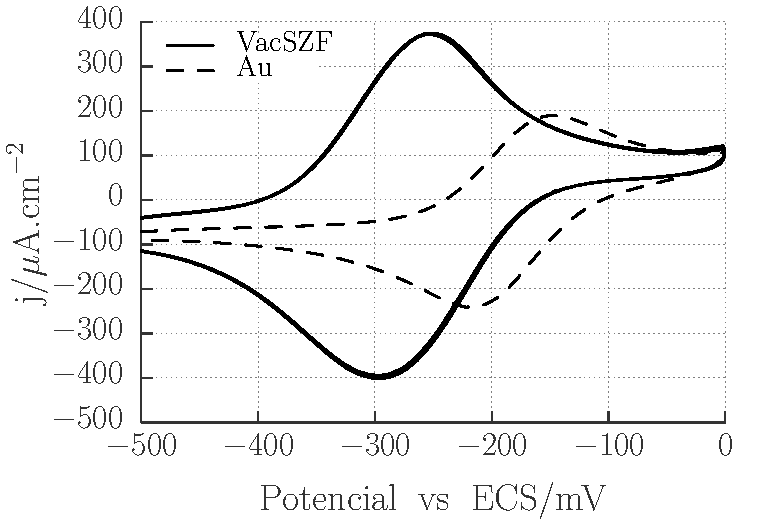
\includegraphics[width=1\textwidth]{Graficos/Zr-Ru1mM-181-246Ciclos.pdf}
			        	\vspace*{-0.40cm}\caption{VCs consecutivas para  \ru\space \SI{1}{\milli\Molar}. Voltagramas grises sobre \pdmZ\space y rojo sobre Au\index{oro} desnudo.}
			        	\label{fig:zr-comp-b}
			         	\end{subfigure}
			         	\caption[Estabilidad de las \pdmZ]{Gráficos para evaluar la estabilidad de las películas \pdmZ\space. a) Comparación en intensidad con \pdmF. b) Voltagramas consecutivos correspondientes a los ciclos 180 al 250 donde se observa que son prácticamente equivalentes.}
			         	\label{fig:zr-comp}
			     	\end{figure}		

\section{Conclusiones parciales}
	
	Durante los capítulos previos se han estudiado y desarrollado métodos para depositar películas delgadas mesoporosa\index{película!mesoporosa} de oxido de silicio\index{silicio!oxido de}\index{silicio} sobre electrodos de Au\index{electrodo!de Au}. A su vez se idearon mecanismos de condensación\index{condensación} y extracción\index{extracción} del surfactante\index{surfactante} a temperaturas por debajo de los \SI{130}{\celsius}. 

	Una vez terminadas estas etapas, se realizó un exhaustivo estudio de las diferentes respuestas electroquímica\index{electroquimico} en función de las interacciones de las \pdm\space con las sonda\index{sonda}s utilizadas. Se verificó la exclusión de sonda\index{sonda}s negativas, la permeación\index{permeacion} de sonda\index{sonda}s neutras y la adsorción\index{adsorción} de las positivas. Los resultados sobre estas últimas nos permitieron, por primera vez, obtener concentraciones dentro de las películas, evaluar la capacidad de preconcetración, estimar la constante de Langmuir\index{Langmuir} y calcular valores de coeficientes de difusión\index{difusión}, ya por trasferencia de masa (como en el caso del \fc) o por transferencia de carga vía \textit{electron hopping}\index{electron hopping@\textit{electron hopping}}, como en el caso del \ru.

	Se simularon voltametrás cíclicas por elementos finitos para interpretar resultados de un experimentos de mediación\index{mediacion} redox, donde se intentaba mediar la respuesta electroquímica\index{electroquimico} de una sonda\index{sonda} a través de una \pdm\space sutura con \ru. Se establecieron las condiciones de contorno para las cuales se podría dar o no dicho proceso y, avanzando con las simulaciones, se pudo establecer si el fenómeno dominante es la mediación\index{mediacion} o la permeación. Se realizó un análisis más general donde se establecen cuales son los procesos que podrían tener lugar dentro de las películas porosas ariando el coeficiente de difusión\index{difusión} y constante de mediación\index{mediacion} redox.

	Se demostró la disolución por completo de las \pdmF\space al ser sometida a varias voltamperometrías consecutivas. Este comportamiento se ha verificado para cualquier tipo de película (ya sea calcinada o no, sobre ITO o sobre Au), pero solo se dá cuando está adsorbido el \aminorutenio y luego de algunos ciclos (con 100 ciclos se disuelve completamente en la mayoría de los casos). Este fenómeno se ha interpretado como una catálisis debida a la migración de iones y contraiones entre la película y la solución. Por último, y no menos importante, se sintetizaron películas delgadas mesoporosas mixtas de óxido de circonio/silicio (\pdmZ), con el método de alto vacio\index{alto@alto vacío} (desarrollado en este mismo trabajo) y con las mismas capacidades selectivas (exclusión, permeación\index{permeacion} y preconcentración) que las de silcio, pero con una resistencia química/mecánica mucho mejor, pudiéndose llevar a cabo hasta 600 ciclos de mediciones con una disminución del 20\% de la señal.


% 	Aca Hay que poner los graficos de 1mM de Ru para INTI\index{INTI} baja T y CNEA\index{CNEA} calcinado donde se muestra y se pueden vislumbrar los dos mecanismos de transporte\index{transporte} de carga, el de libre y el Ru adsorbido.!!!!

% 	Agragar todo lo del ferroceno, lo catalisis con HQ y tambien la mediacion con ferro/ferri

% 	Hay que tener en cuenta aqui el tema de la respuesta Eq que solo son sitios activos los adsorbido y que puede que haya mas Rutenio adsorbido en realiadad. Es una cota inferior de la concentracion dentro de lo poros. Además esta el tema del area, trabajamos siempre con el area geometrica pero se sabe que esta no es el area del electrodo activa sino que es mas..... ambos efectos van en el mismo camino a favor de una mayor concentracion.


%---------------------------------------------------------------------------------------------------------

%HACE FALTA LA CARACTERIZACION COMPLETA DEL MESO SIZR????  y Colocarlo en el capitulo 4???	
%FTIR - SEM\index{SEM} - EPA - CA - EDS???? OPTICO

%Reemplazar los valores de la curva de calibrado y los usado en el adsorbido por numeros redondos, 6, 3, 1.5

%Distancia entre sitios redox\index{sitio redox\index{sitio redox}}
